\let\negmedspace\undefined
\let\negthickspace\undefined
\documentclass[journal]{IEEEtran}
\usepackage[a5paper, margin=10mm, onecolumn]{geometry}
\usepackage{tfrupee}

\setlength{\headheight}{1cm}
\setlength{\headsep}{0mm}

\usepackage{gvv-book}
\usepackage{gvv}
\usepackage{cite}
\usepackage{amsmath,amssymb,amsfonts,amsthm}
\usepackage{algorithmic}
\usepackage{graphicx}
\usepackage{textcomp}
\usepackage{xcolor}
\usepackage{txfonts}
\usepackage{listings}
\usepackage{enumitem}
\usepackage{mathtools}
\usepackage{gensymb}
\usepackage{comment}
\usepackage[breaklinks=true]{hyperref}
\usepackage{tkz-euclide}
\usepackage{listings}
\def\inputGnumericTable{}
\usepackage[latin1]{inputenc}
\usepackage{color}
\usepackage{array}
\usepackage{longtable}
\usepackage{calc}
\usepackage{multirow}
\usepackage{hhline}
\usepackage{ifthen}
\usepackage{lscape}

\begin{document}

\bibliographystyle{IEEEtran}
\vspace{3cm}

\title{5.2.6}
\author{EE25BTECH11003 - Adharvan Kshathriya Bommagani}
{\newpage\maketitle}

\renewcommand{\thefigure}{\theenumi}
\renewcommand{\thetable}{\theenumi}
\setlength{\intextsep}{10pt}

\textbf{Question}:\\
Solve the following system of linear equations using Gaussian elimination and matrices:
\begin{center}
    2x - 3y = 8 \\
    4x - 6y = 9
\end{center}

\bigskip

\textbf{Solution}:\\

First, we represent the system of equations as an augmented matrix. 
\begin{align}
\myaugvec{2}{
2 & -3 & 8 \\
4 & -6 & 9
}
\end{align}

Apply the row operation $R_2 \to R_2 - 2R_1$:
\begin{align}
\myaugvec{2}{
2 & -3 & 8 \\
0 & 0 & -7
}
\end{align}
Now, we translate the second row of the resulting matrix back into an equation:
\begin{align}
    0x + 0y = -7
\end{align}
This simplifies to the statement:
\begin{align}
    0 = -7
\end{align}
This statement is a contradiction, as 0 is not equal -7.

Because the process leads to a contradiction, the original system of equations is described as \textbf{inconsistent}. This means there is no pair of values for $x$ and $y$ that can satisfy both equations simultaneously. Therefore, the system has \textbf{no solution}.
\newpage

\textbf{Plot of the Lines:}
\begin{figure}[H]
    \centering
    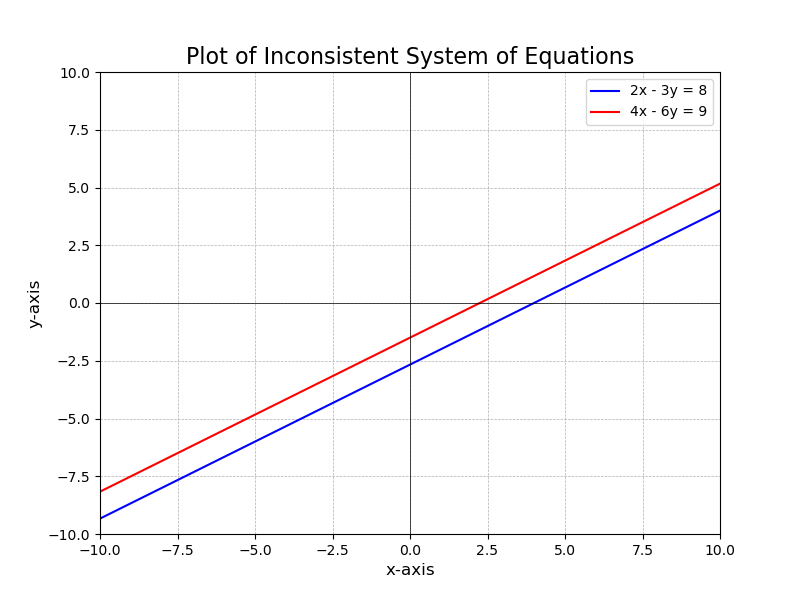
\includegraphics[width=0.9\columnwidth]{figs/fig1.png}
    \caption{Figure for 5.2.6}
    \label{}
\end{figure}


\end{document}